% !TeX encoding = UTF-8

\documentclass{protokol}

\usepackage{pdfpages}
\usepackage{tikz}
\usetikzlibrary{calc}
\usetikzlibrary{arrows}

%====== Units =====
\usepackage{siunitx}
\sisetup{inter-unit-product =\ensuremath{\cdot}}
\sisetup{group-digits = integer}
\sisetup{output-decimal-marker = {,}}
\sisetup{exponent-product = \ensuremath{\cdot}}
\sisetup{separate-uncertainty}
\sisetup{tight-spacing = false}
%\sisetup{scientific-notation = true}
%\sisetup{round-mode=places,round-precision=4}
%\sisetup{evaluate-expression}


%====== Grafy =====
\usepackage{pgfplots}
\pgfplotsset{width=0.8\linewidth, compat=1.17}
\def\plotcscale{0.8}
\usepackage{pgfplotstable}
\usepackage[figurename=Obr.]{caption} % figure caption rename

%====== Rovnice align block ======
\usepackage{amsmath}
\setlength{\jot}{10pt} % rozestup mezi řádky

\graphicspath{ {./img/} }

%====== Vyplňte údaje ======
\jmeno{Jakub Charvot}
\kod{240844}
\rocnik{3.}
\obor{MET}
\skupina{MET/2}
\spolupracoval{--}

\merenodne{5.12.\ 2023}
\odevzdanodne{5.12.\ 2023}
\nazev{Měření a dostavování rezistorů}
\cislo{6} %měřené úlohy

\predmet{Mikroelektronika a technologie součástek}
\ustav{Ústav mikroelektroniky}
\skola{FEKT VUT v~Brně}

\def\para{x+0}
\def\parb{\para-80}


%citace 
\usepackage[backend=biber, style=iso-numeric, sortlocale=cs_CZ, autolang=other, language=czech]{biblatex}
\addbibresource{bibliography.bib}
\DeclareFieldFormat{labelnumberwidth}{\mkbibbrackets{#1}}
% hyperlinky
\usepackage[colorlinks]{hyperref}

% odstavce
\usepackage{parskip}

% Bloky kódu
\usepackage{xcolor}

%New colors defined below
\definecolor{codegreen}{rgb}{0,0.6,0}
\definecolor{codegray}{rgb}{0.5,0.5,0.5}
\definecolor{codepurple}{rgb}{0.58,0,0.82}
\definecolor{backcolour}{rgb}{0.95,0.95,0.92}

\usepackage{listings}
\lstdefinestyle{mystyle}{
  backgroundcolor=\color{backcolour}, commentstyle=\color{codegreen},
  keywordstyle=\color{magenta},
  numberstyle=\tiny\color{codegray},
  stringstyle=\color{codepurple},
  basicstyle=\ttfamily\footnotesize,
  breakatwhitespace=false,         
  breaklines=true,                 
  captionpos=b,                    
  keepspaces=true,                 
  numbers=left,                    
  numbersep=5pt,                  
  showspaces=false,                
  showstringspaces=false,
  showtabs=false,                  
  tabsize=2
}
\lstset{
	inputencoding=utf8,
	extendedchars=true,
	literate={á}{{\'a}}1 {č}{{\v{c}}}1 {ď}{{\v{d}}}1 {é}{{\'e}}1 {ě}{{\v{e}}}1 
           {í}{{\'i}}1 {ň}{{\v{n}}}1 {ó}{{\'o}}1 {ř}{{\v{r}}}1 {š}{{\v{s}}}1 
           {ť}{{\v{t}}}1 {ú}{{\'u}}1 {ů}{{\r{u}}}1 {ý}{{\'y}}1 {ž}{{\v{z}}}1 
           {Á}{{\'A}}1 {Č}{{\v{C}}}1 {Ď}{{\v{D}}}1 {É}{{\'E}}1 {Ě}{{\v{E}}}1 
           {Í}{{\'I}}1 {Ň}{{\v{N}}}1 {Ó}{{\'O}}1 {Ř}{{\v{R}}}1 {Š}{{\v{S}}}1 
           {Ť}{{\v{T}}}1 {Ú}{{\'U}}1 {Ů}{{\r{U}}}1 {Ý}{{\'Y}}1 {Ž}{{\v{Z}}}1,
	style=mystyle
	}

% Číslování
\pagenumbering{arabic}

% =========================================
% =============== DOKUMENT ================
% =========================================
\begin{document}
	%====== Vygenerování tabulky ======
	\maketitle

\section{Teoretický úvod}
  Teorie potřebná k této úloze vychází z předešlých laboratorních úloh, zejména úlohy 2, kdy jsme měřili hodnoty tlustovrstvých rezistorů v závislosti na různých podobách výpalu a také změnu jejich odporu v závislosti na teplotě. Přijde mi zbytečné uvádět znovu základní informace o samotné technologii nebo výpočtu odporu na čtverec, které již v této době semestru musí znát opravdu každý student, proto bude tato sekce o něco kratší.

\subsection{Dostavování TLV rezistorů}
Co se týče nové teorie věnuje se tato úloha také dostavování (nebo také trimmování) již natištěných rezistorů. 
Jak jsme si již vyzkoušeli na předchozích úlohách, přesnost tisku je velkou neznámou a i při optimalizaci všech dostupných parametrů jsou hodnoty stále poměrně nepřesné. Z tohoto důvodu se s nepřesností v návrhu počítá a tisknou se rezistory s o něco nižšími hodnotami než je požadováno. Následně jsou rezistory měřeny a v průběhu měření je jich část odebrána tak, aby se svou hodnotou více přiblížili požadavku. 

Nejčastějšími způsoby je mechanické osbroušení, obvykle proudem částic korundu nebo křemíku, nebo odpaření vrstvy laserem, většinou typ YAG nebo CO\(_{2}\). 

Pro dostavení je možné vyřezat do tlustovrstvého motivu různé obrazce. Obvykle se volí přímý řez od kraje směrem ke středu. Pokud se takovýchto provede více vedle a naproti sobě, vznikne serpentýnový motiv. Alternativou je ještě výřez ve tvaru L \cite{zadani,schroeder2022trimming}.

\section{Praktická část}
  Měřili jsme hodnoty odporů vytvořených technologií tlusté vrstvy na testovacím substrátu, viz obr.~\ref{fig:img-fuck-png}. Na substrátu byl uvedený motiv 4x a to vždy pootočen o \qty{90}{\degree}, díky takovému měření je pak teoreticky možné stanovit vliv různých parametrů tisku TLV, zejména ověřit, jestli je tisk homogenní v obou osách. Na základě měření je pak možné upravit parametry tisku tak, aby při tisku skutečného integrovaného obvodu byl výsledek co nejvíce optimální a předvídatelný. 

Všechny měřené hodnoty se nachází v tabulce, která je pro lepší přehlednost umístěna až na samotném konci dokumentu. 

\subsection{Zpracování měřených dat}
    Na základě pokynů vyučujícího byla stanovena teoretická hodnota odporu (viz zmíněná tabulka). Vypočtena byla následovně:
    \[
        R_{teor}  = R_{sq}\cdot \frac{L}{W} 
    \]
    Ačkoliv toto nebylo vyučujícím upřesněno, předpokládaná jednotka zadaných rozměrů jsou \unit{\micro\meter}. Z nám dodaných údajů vyplývá, že byla použita odporová pasta s odporem \qty{100}{\ohm\per sq}.

    Následně byla do grafu vynesena závislost odporu na délce rezistoru. Byl vytvořen graf pro každou odporovou sérii a nachází se v něm data ze všech čtyř kvadrantů, pro jednotlivé série se jedná o grafy \ref{graf:RX-1}, \ref{graf:RX-2}, \ref{graf:RX-3} a \ref{graf:RX-4}.

\begin{figure}[h!]
    \centering
    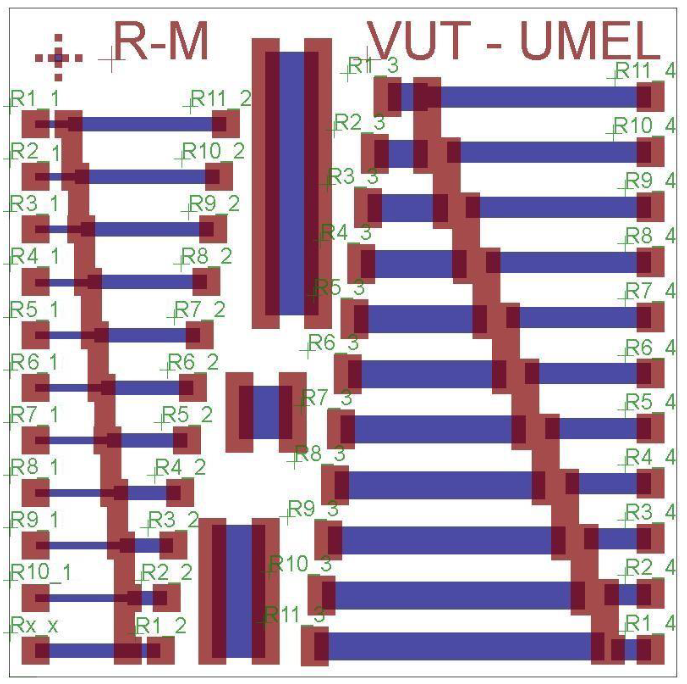
\includegraphics[width=0.5\textwidth]{img/fuck.png}
    \caption{Testovací substrát. Převzato z~\cite{zadani}.}
    \label{fig:img-fuck-png}
\end{figure}

\begin{figure*}[h!]
    \begin{tikzpicture}
        \centering
        \begin{axis}
            [
            xlabel={\( L\ [\unit{\micro\meter}]\)},
            ylabel={\( R\ [\unit{\mega\ohm}]\)},
            %axis y line*=left, % dve y osy
            width=1\textwidth,
            height = 0.5\textwidth,
            legend pos=north west,
%			xmin=0,
%			ymin=0,
%			xmax=100
%			ymax=100
            ]

            \addplot[mark=x, mark options={solid}, thick,  red,   mark size=3pt] table [skip first n=0, x=delka,   y=Q1, col sep=comma] {data/ser1.csv};
            \addlegendentry{RX\_1 Q1}
            \addplot[mark=x, mark options={solid}, thick,  green, mark size=3pt] table [skip first n=0, x=delka, y=Q2, col sep=comma] {data/ser1.csv};
            \addlegendentry{RX\_1 Q2}
            \addplot[mark=x, mark options={solid}, thick,  blue,  mark size=3pt] table [skip first n=0, x=delka,  y=Q3, col sep=comma] {data/ser1.csv};
            \addlegendentry{RX\_1 Q3}
            \addplot[mark=x, mark options={solid}, thick,  black, mark size=3pt] table [skip first n=0, x=delka, y=Q4, col sep=comma] {data/ser1.csv};
            \addlegendentry{RX\_1 Q4}
            
            
        \end{axis}   
    \end{tikzpicture}
    \caption{Závislost odporu na délce. Série RX\_1.}
    \label{graf:RX-1}
\end{figure*}

\begin{figure*}[h!]
    \begin{tikzpicture}
        \centering
        \begin{axis}
            [
            xlabel={\( L\ [\unit{\micro\meter}]\)},
            ylabel={\( R\ [\unit{\mega\ohm}]\)},
            %axis y line*=left, % dve y osy
            width=1\textwidth,
            height = 0.5\textwidth,
            legend pos=north west,
%			xmin=0,
%			ymin=0,
%			xmax=100
%			ymax=100
            ]

            \addplot[mark=x, mark options={solid}, thick,  red,   mark size=3pt] table [skip first n=0, x=delka,   y=Q1, col sep=comma] {data/ser2.csv};
            \addlegendentry{RX\_2 Q1}
            \addplot[mark=x, mark options={solid}, thick,  green, mark size=3pt] table [skip first n=0, x=delka, y=Q2, col sep=comma] {data/ser2.csv};
            \addlegendentry{RX\_2 Q2}
            \addplot[mark=x, mark options={solid}, thick,  blue,  mark size=3pt] table [skip first n=0, x=delka,  y=Q3, col sep=comma] {data/ser2.csv};
            \addlegendentry{RX\_2 Q3}
            \addplot[mark=x, mark options={solid}, thick,  black, mark size=3pt] table [skip first n=0, x=delka, y=Q4, col sep=comma] {data/ser2.csv};
            \addlegendentry{RX\_2 Q4}
            
            
        \end{axis}   
    \end{tikzpicture}
    \caption{Závislost odporu na délce. Série RX\_2.}
    \label{graf:RX-2}
\end{figure*}

\begin{figure*}[h!]
    \begin{tikzpicture}
        \centering
        \begin{axis}
            [
            xlabel={\( L\ [\unit{\micro\meter}]\)},
            ylabel={\( R\ [\unit{\mega\ohm}]\)},
            %axis y line*=left, % dve y osy
            width=1\textwidth,
            height = 0.5\textwidth,
            legend pos=north west,
%			xmin=0,
%			ymin=0,
%			xmax=100
%			ymax=100
            ]

            \addplot[mark=x, mark options={solid}, thick,  red,   mark size=3pt] table [skip first n=0, x=delka,   y=Q1, col sep=comma] {data/ser3.csv};
            \addlegendentry{RX\_3 Q1}
            \addplot[mark=x, mark options={solid}, thick,  green, mark size=3pt] table [skip first n=0, x=delka, y=Q2, col sep=comma] {data/ser3.csv};
            \addlegendentry{RX\_3 Q2}
            \addplot[mark=x, mark options={solid}, thick,  blue,  mark size=3pt] table [skip first n=0, x=delka,  y=Q3, col sep=comma] {data/ser3.csv};
            \addlegendentry{RX\_3 Q3}
            \addplot[mark=x, mark options={solid}, thick,  black, mark size=3pt] table [skip first n=0, x=delka, y=Q4, col sep=comma] {data/ser3.csv};
            \addlegendentry{RX\_3 Q4}
            
            
        \end{axis}   
    \end{tikzpicture}
    \caption{Závislost odporu na délce. Série RX\_3.}
    \label{graf:RX-3}
\end{figure*}

\begin{figure*}[h!]
    \begin{tikzpicture}
        \centering
        \begin{axis}
            [
            xlabel={\( L\ [\unit{\micro\meter}]\)},
            ylabel={\( R\ [\unit{\mega\ohm}]\)},
            %axis y line*=left, % dve y osy
            width=1\textwidth,
            height = 0.5\textwidth,
            legend pos=north west,
%			xmin=0,
%			ymin=0,
%			xmax=100
%			ymax=100
            ]

            \addplot[mark=x, mark options={solid}, thick,  red,   mark size=3pt] table [skip first n=0, x=delka,   y=Q1, col sep=comma] {data/ser4.csv};
            \addlegendentry{RX\_4 Q1}
            \addplot[mark=x, mark options={solid}, thick,  green, mark size=3pt] table [skip first n=0, x=delka, y=Q2, col sep=comma] {data/ser4.csv};
            \addlegendentry{RX\_4 Q2}
            \addplot[mark=x, mark options={solid}, thick,  blue,  mark size=3pt] table [skip first n=0, x=delka,  y=Q3, col sep=comma] {data/ser4.csv};
            \addlegendentry{RX\_4 Q3}
            \addplot[mark=x, mark options={solid}, thick,  black, mark size=3pt] table [skip first n=0, x=delka, y=Q4, col sep=comma] {data/ser4.csv};
            \addlegendentry{RX\_4 Q4}
            
            
        \end{axis}   
    \end{tikzpicture}
    \caption{Závislost odporu na délce. Série RX\_4.}
    \label{graf:RX-4}
\end{figure*}

  \clearpage

\section{Závěr}
  Jak je vidět z grafů a tubulky naměřených hodnot, pro některé série jsou výsledky v různých kvadrantech obdobné, pro některé naopak vůbec. Nejhomogennějšíh výsledku dosáhla série RX\_3. Také je vidět, že napříč sériemi vycházely celkově o něco menší hodnoty v prvním kvadrantu a naopak vyšší ve druhém a třetím. 

Při porovnání naměřených hodnot s teoretickými se ale dostáváme do prekérní situace. Odchylka zde dosahuje několika řádů kdy namísto stovek \unit{\ohm} měříme hodnoty i v nižších stovkách \unit{\mega\ohm}, typycky pak v jednotkách \unit{\mega\ohm}. Toto nasvědčuje buďto hrubé systematické chybě měření neno špatným informacím ohledně použité odporové pasty, popř. kombinaci obou faktorů. Vzhledem k tomu, že měření bylo prováděno poměrně dlouhý čas a dohlíženo čtyřmi osobami se mi takto hruhá chyba jeví jako nepravděpodobná, ovšem vyloučna není. 
  
\clearpage
\section*{Reference}
\printbibliography[heading=none]

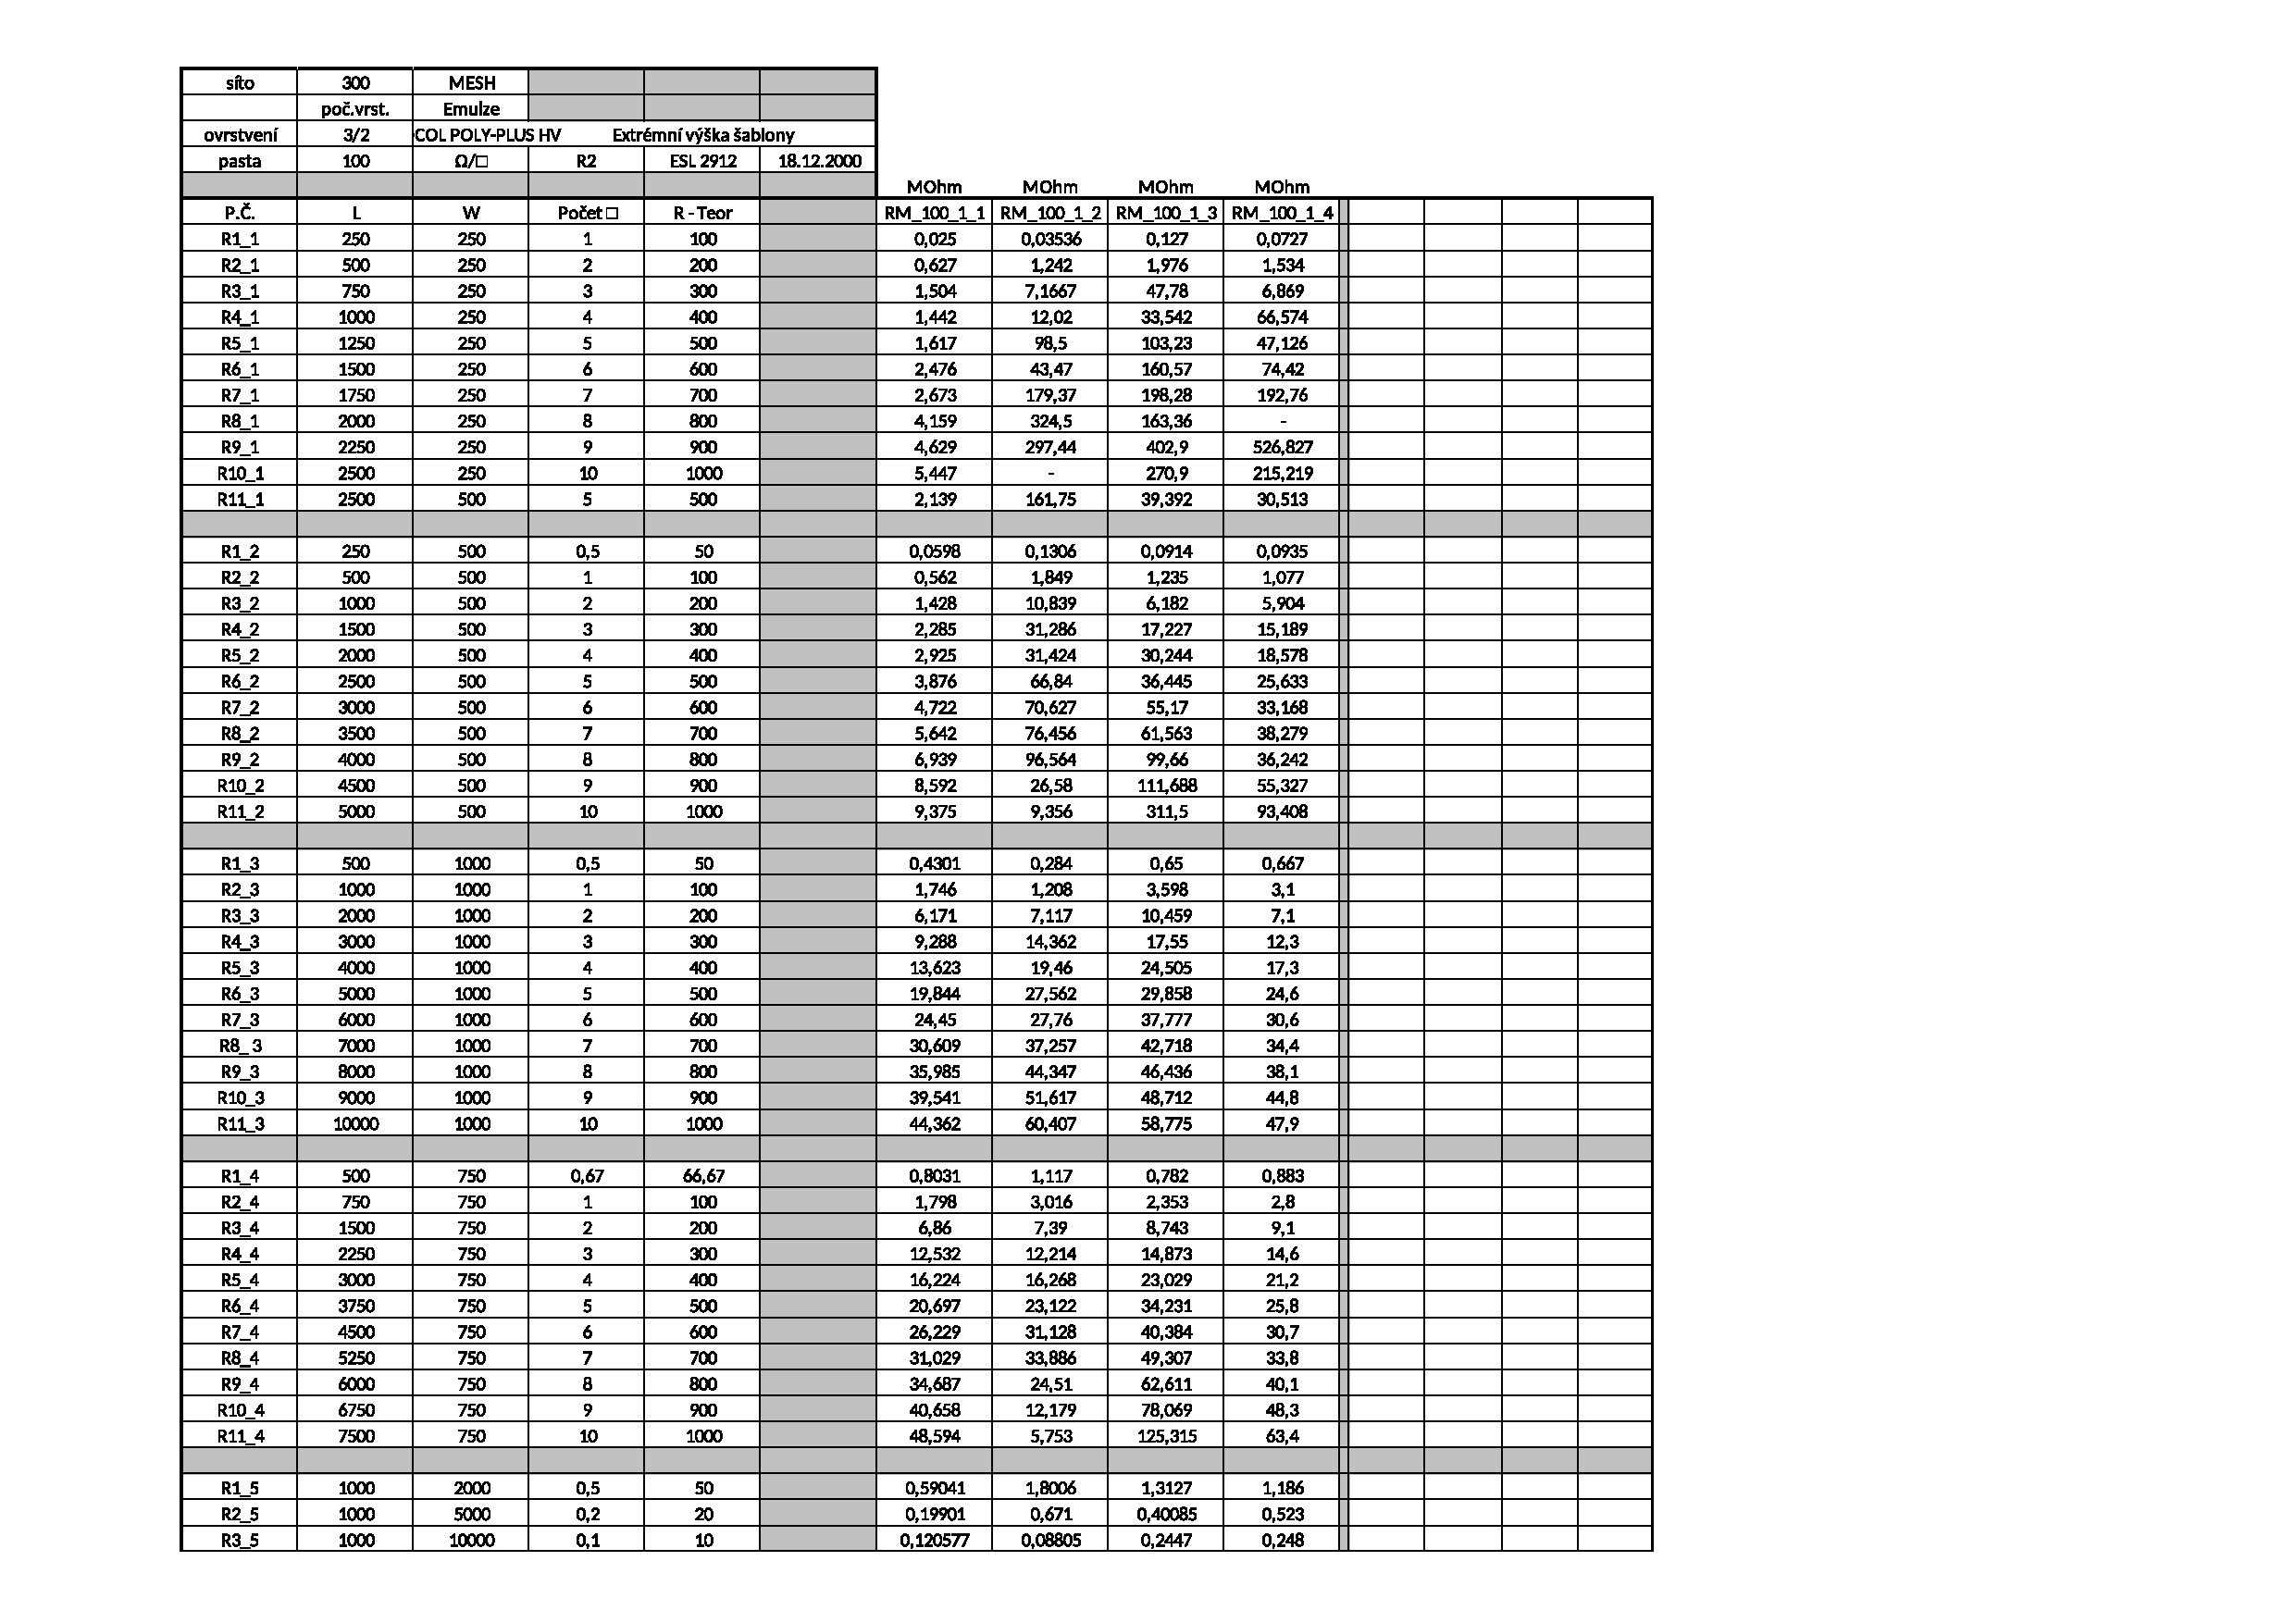
\includepdf[pages=1]{data/data.pdf}

\end{document}